%!TEX root = ../thesis.tex
% ******************************* Thesis Appendix B ****************************
\chapter{Nonparametric copula estimation}
\label{apx:B}
%*******************************************************************************

\elias{update CDF notations}

\elias{Change EBC notations using h for the polynomial orders}

When the distribution's dimension is higher than two, one can perform a parametric fit using vine copulas \citep{joe2011dependence}, implying the choice of multiple types of parametric copulas. 
Otherwise, nonparametric fit by multivariate kernel density estimation (KDE) presents a computational burden as soon as the dimension increases \citep{chabridon2021global}. 
Since univariate marginals are usually well-fitted with nonparametric tools (e.g., KDE), let us introduce an effective nonparametric method for copula fitting.

%============================================================%
\section{Empirical copula}
%============================================================%
In practice, considering a sample $\bX_n = \left\{\bx^{(1)}, \dots, \bx^{(n)}\right\} \in \R^{np}$ and the associated ranked sample $\bR_n = \left\{\br^{(1)}, \dots, \br^{(n)}\right\}$, the corresponding empirical copula writes: 
\begin{equation}
    C_n(\bu) := \frac1n \sum_{i=0}^{n} \prod_{j=1}^{p} \1 \left\{ \frac{r_j^{(i)}}{n} \leq u_j \right\},
\end{equation}
with $\bu = (u_1, \dots, u_d) \in [0, 1]^d$. In the following, the polynomial order is set as equal in each dimension: $\{m_i = m\}_{j=1}^d$. 

%============================================================%
\section{Empirical Bernstein \& Beta copula}
%============================================================%

Copulas are continuous and bounded functions defined on a compact set (the unit hypercube). 
Bernstein polynomials allow us to uniformly approximate as closely as desired any continuous and real-valued function defined on a compact set (Weierstrass approximation theorem). 
Therefore, they are good candidates to approximate unknown copulas. 
This concept was introduced as \emph{empirical Bernstein copula} (EBC) by \cite{sancetta_satchell_2004} for applications in economics and risk management. 
Later on, \cite{segers_2017} offered further asymptotic studies. 
Formally, the multivariate Bernstein polynomial for a function $C: [0, 1]^d \rightarrow \R$ on a grid over the unit hypercube $G:=\left\{\frac{0}{m_1}, \dots, \frac{m_1}{m_1}\right\} \times \dots \times \left\{\frac{0}{m_d}, \dots, \frac{m_d}{m_d}\right\}, \bm = (m_1, \dots, m_d) \in \N^d$, writes: 
\begin{equation}
    B_{\bm}(C)(\bu) := \sum_{t_1=0}^{m_1} \dots \sum_{t_d=0}^{m_d} C\left(\frac{t_1}{m_1}, \dots, \frac{t_d}{m_d}\right) \prod_{j=1}^d P_{m_j, t_j}(u_j),\label{eq:ebc}
\end{equation}
with $\bu = (u_1, \dots, u_d) \in [0, 1]^d$, and the Bernstein polynomial $P_{m, t}(u):= \frac{t!}{m!(t-m)!}u^m(1-u)^{t-m}$. 
Notice how the grid definition implies the polynomial's order. 
When $C$ is a copula, then $B_{\bm}(C)$ is called ``Bernstein copula''. 
Therefore, the empirical Bernstein copula is an application of the Bernstein polynomial in \eq{eq:ebc} to the so-called ``empirical copula''.
\elias{add a sentence to mean to refer to the previous subsection}

Theoretically, the tuning parameter can be optimized to minimize an ``Mean Integrated Squared Error'' (MISE), leading to a bias-variance tradeoff. 
Formally, the MISE of the empirical Bernstein copula $B_{\bm}(C_n)$ is defined as follows:
\begin{equation}
    \E\!\left[ \lVert B_{\bm}(C_n) - C \rVert^2_2 \right] \!=\! \E\!\left[\!\int_{\R^d}\! \left(B_{\bm}(C_n)(\bu) \!-\! C(\bu) \d \bu \right)^2 \!\right]\!\!.
    \label{eq:kimse}
\end{equation}
Then, \cite{sancetta_satchell_2004} prove in their Theorem 3 that: 
\begin{itemize}
    \item $B_{\bm}(C_n)(\bu) \rightarrow C(\bu)$ for any $u_j \in \left]0, 1\right[$ if $\frac{m^{d/2}}{n} \rightarrow 0$, when $m, n \rightarrow \infty$.
    \item The optimal order of the polynomial in terms of MISE is: $m \lesssim m_{\mathrm{IMSE}} = n^{2/(d+4)}, \forall u_j \in \left]0, 1\right[$. The sign $\lesssim$ means ``less than or approximately''.
\end{itemize}

Let us remark that in the special case $m = n$, also called the ``Beta copula'' in \cite{segers_2017}, the bias is very small while the variance gets large. 
To illustrate the previous theorem, \cite{lasserre_2022} represents the evolution of the $m_{\mathrm{IMSE}}$ for different dimensions and sample sizes (see \fig{fig:hmise}). 
In high dimension, the values of $m_{\mathrm{IMSE}}$ tend towards one, which is equivalent to the independent copula. 
Therefore, high-dimensional problems should be divided into a product of smaller problems on which the EBC is tractable. 
Provided a large enough learning set $\bX_n$, KDE fitting of marginals combined with EBC fitting of the copula delivers good results even on complex dependence structures. 
Moreover, EBC provides an explicit expression, making a Monte Carlo generation of i.i.d. samples simple. 

\begin{figure}
    \centering
    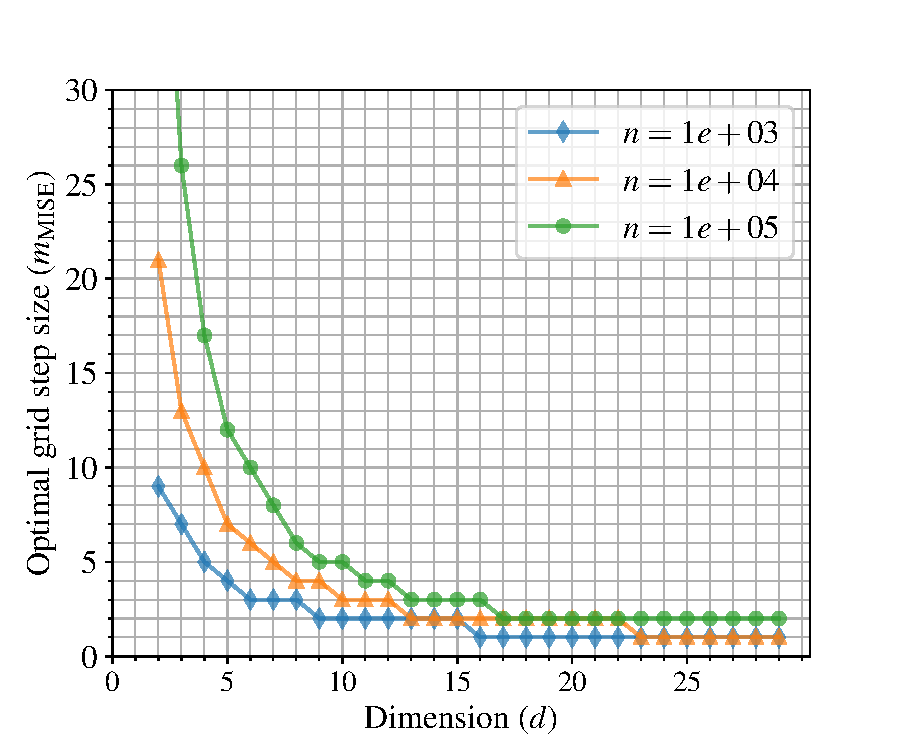
\includegraphics[width=0.6\linewidth]{part3/figures/BANCS/hMISE.pdf}
    \caption{Evolution of $m_{\mathrm{IMSE}}$ for different dimensions and sample sizes.}
    \label{fig:hmise}
\end{figure}


%============================================================%
\section{Goodness-of-fit}
%============================================================%


\elias{Mention the vine copulas and how we want to only use nonparametric methods here.}

\elias{Tails correlation / Kendall plot}